\documentclass[11pt]{paper}
\usepackage{gary}
\usepackage{subfigure}
\usepackage[margin=1in]{geometry}
\usepackage{mwe}
\usepackage{biblatex}
\addbibresource{stat153_project_report.bib}
\title{Modeling Frequency of Terrorist Attacks}
\author{Gary Cheng and Preetham Gujjula}
\date{\today}

\begin{document}
\maketitle 

\section{Introduction}
Global terrorism is a major issue today, and has been in the American zeitgeist at least since 9/11. Identifying patterns in attacks, and being able to predict future attacks, would be useful to law enforcement and the public. For these reasons, we decided to use this project as an opportunity to study a dataset of terrorist attacks from around the world.

The dataset we chose is the Global Terrorism Database, compiled by the National Consortium for the Study of Terrorism and Responses to Terrorism (START), located at the University of Maryland, College Park. START published the GTD on Kaggle, which is where we procured the dataset from \cite{kaggle}. The GTD aims to be a comprehensive record of all terrorist attacks, starting from 1970. It collects dozens of variables for each attack, including date, country, target, perpetrator, tactic used, weapons used, casualties, and fatalities \cite{gtdmethodology}.

We wanted to use the GTD to study the number of terrorist attacks that occur over time. In particular, we planned to derive a time series dataset from the GTD of the number of terrorist attacks that occur each month. We aimed to fit a model to this time series, and use the model to predict the number of terrorist attacks in the next 12 months. We decided on this duration because it was long enough to be valuable while still being within the prediction capabilities of the SARIMA model.

\section{Data Analysis}
\subsection{Cleaning}

Our uncleaned dataset contains every terrorist attack from 1970 to 2016. To form a time series out of this dataset, we counted the number of attacks that occurred each month and created a vector of these values. Figure \ref{ogogog} in the appendix displays a plot of the number of attacks per month since 1970.

It should be noted that the data from 1998 to 2007 was collected retrospectively, as opposed to the other data, which was collected in real time. According to START, retrospective collection may underestimate the true number of terrorist attacks, because some media sources that documented the attacks are no longer available. Indeed, there is a subtle drop in the number of attacks in Figure \ref{ogogog} for those years.

Furthermore, the GTD broadly defines a terrorist attack as ``the threatened or actual use of illegal force and violence by a non-state actor to attain a political, economic, religious, or social goal through fear, coercion, or intimidation''. This is quite a loose definition, which is understandable, since the GTD aims to be as inclusive as possible, and allow researchers to filter the data according to their own criteria.

For both of the reasons mentioned above, we filtered the original dataset to select attacks that resulted in 10 or more casualties. Our rationale is that the likelihood of under counting terrorist attacks of that magnitude is far less. Furthermore, attacks of this scale are more in line with what a layman would consider a terrorist attack. The plot of the filtered time series is rendered in Figure \ref{og} as the black lines. The definition of terrorist attack we will be working with is:

\begin{mydef}[Terrorist Attack]
The threatened or actual use of illegal force and violence by a non-state actor to attain a political, economic, religious, or social goal through fear, coercion, or intimidation, where the number of causalities is greater than or equal to 10.
\end{mydef}

\begin{figure}
\centering
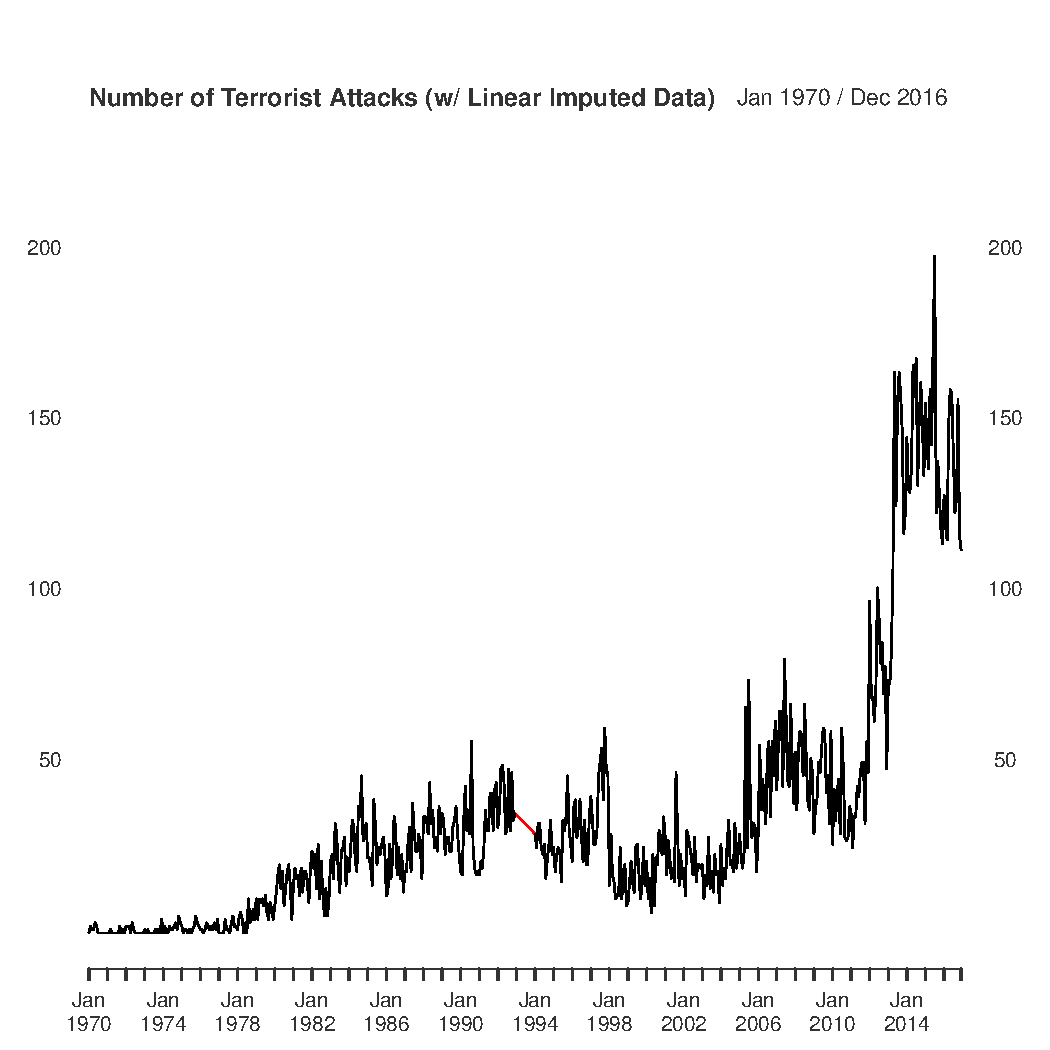
\includegraphics[width=0.75\linewidth]{../image/og_ts.pdf}
\caption{The original time series with a linear imputation (in red) for the missing data in 1993.}
\label{og}
\end{figure}

%\subsection{Interpolation}

There is a gap of 12 missing data points corresponding to the year 1993 because the data, which was collected by the Pinkerton Global Intelligence Service (PGIS), was lost before being transferred to START. To correct for this gap, we impute the data using the tsimpute library in R. In general, selecting an imputation method is difficult because it requires a model of the data first. Furthermore, our data loss was not at random locations but rather clustered together. Thus, we opted to use the simplest imputation method, which patches the missing data with a linear fit. Figure \ref{og} displays the time series with the imputed data in red.

%\subsection{Outliers}

Now we filter outliers from the dataset. Outliers by definition can't be modeled very well, so it is important that they are removed before model building. The library tsoutliers provides a convenient way to identify different kinds of outliers in the dataset. We decided to only filter for additive offset, transient change, and innovational outliers, i.e., outliers manifested as spikes in the underlying dataset. We decided not to filter for level-shift outliers, since we expect to see level-shifts in the timeseries. We also didn’t filter for seasonal additive outliers, since we would not be surprised to see seasonal spikes or dips in the time series.

%\subsection{Final raw Time Series}
After filtering for 10 casualties, imputing the data, and removing outliers, the time series that we will be working can be found in Figure \ref{outlier}. The outlier effects detected can be viewed in Figure \ref{outlier_effect} in the appendix.

\begin{figure}
\centering
    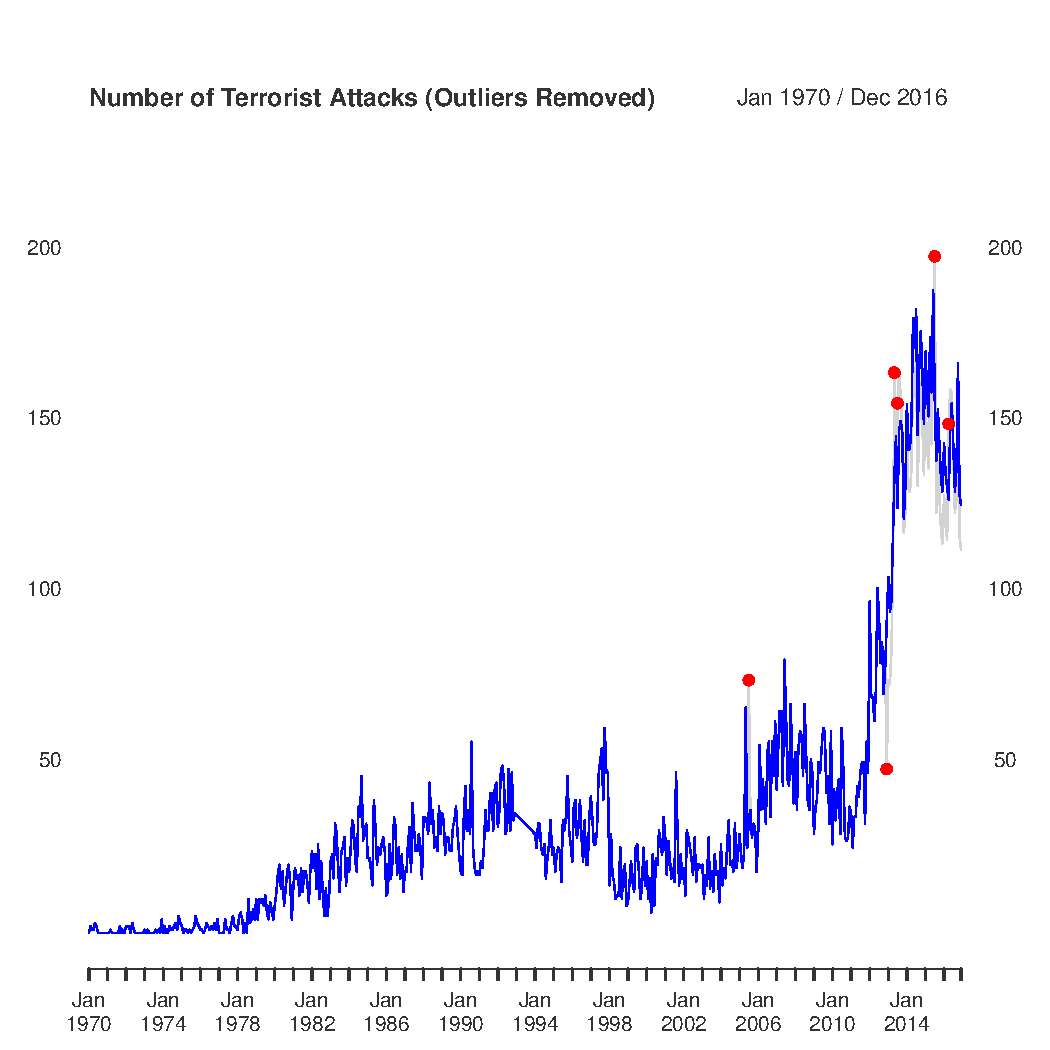
\includegraphics[width=0.75\textwidth]{../image/outlier_comparison.pdf}
\caption{The imputed time series (in blue) with outliers removed. The original time series shown in gray. The 6 outliers are shown in red. }
\label{outlier}
\end{figure}

For purposes of model selection and cross-validation, we split our dataset into three disjoint components: training, validation, and testing. The training dataset was used to find candidate models. The validation dataset was then used to select the best candidate model. Then finally, the testing dataset was used as a final assessment of how well our selected model performs. It should be noted that these components are made disjoint to ensure that we do not bias the model to overfit on testing data. Furthermore, the components are sequential blocks, with the training set consisting of data from 1970-2012 inclusive, the validation from 2013-2015 inclusive, and the testing from the year 2016.


\subsection{Chasing Stationarity}
Visually, the original timeseries does not seem stationary. In particular, the mean of the series appears to increase as time progresses. In addition, the ACF and the PACF of the timeseries, plotted in Figure \ref{og_acf_pacf}, decays slowly as the lag increases---another indication that the series is not stationary.

\begin{figure}
\centering
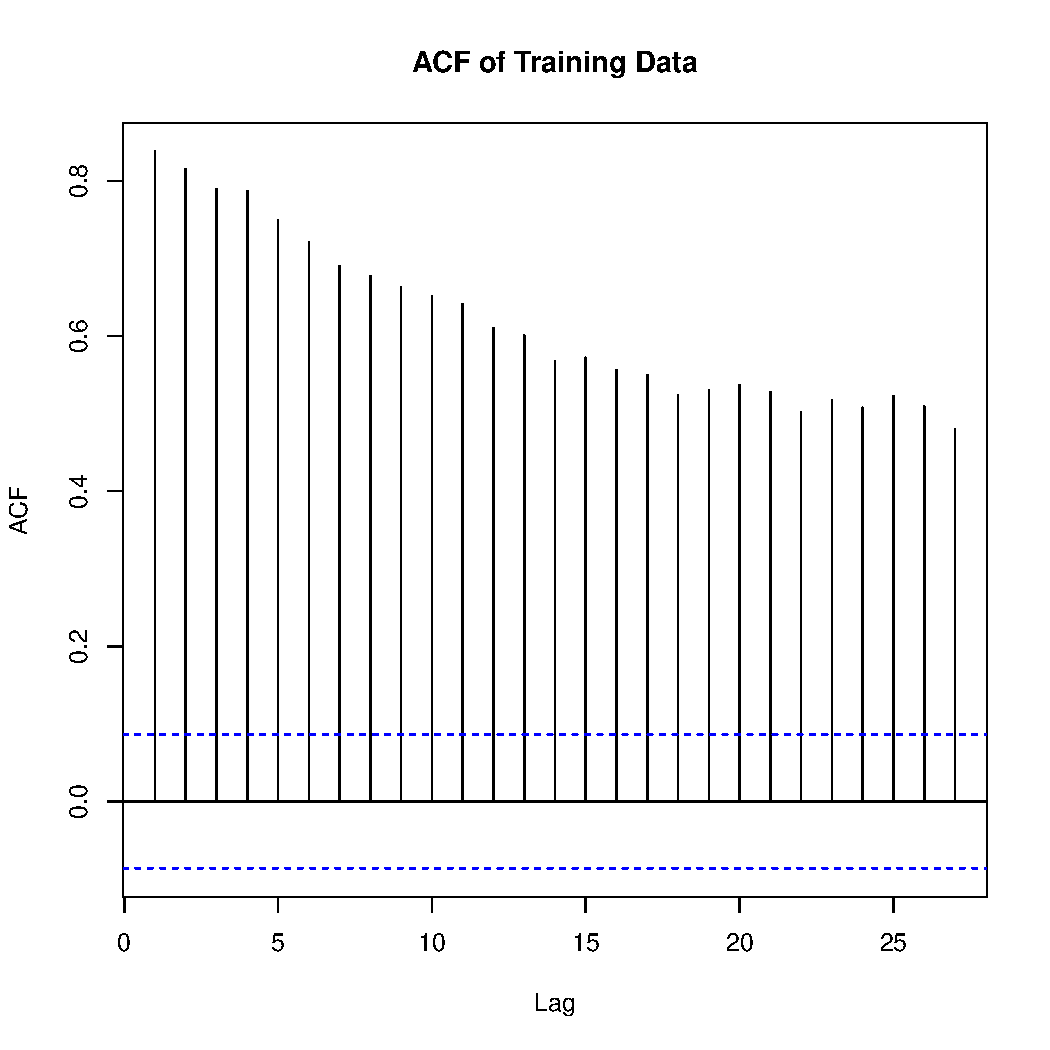
\includegraphics[width=0.45\linewidth]{../image/acf_og.pdf}
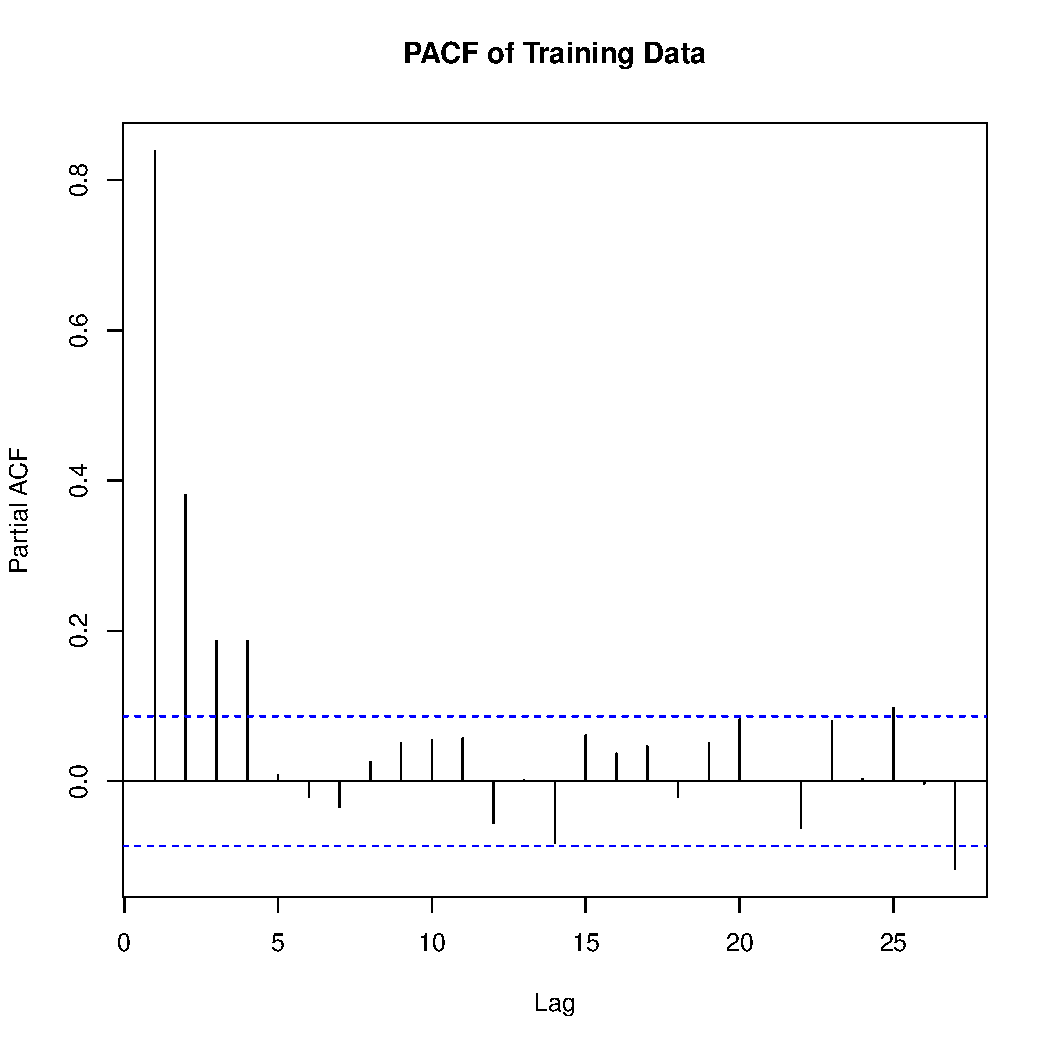
\includegraphics[width=0.45\linewidth]{../image/pacf_og.pdf}
\caption{The ACF and PACF of the time series}
\label{og_acf_pacf}
\end{figure}


%\subsection{Logged Data}

One potential method to derive a stationary timeseries is to take the log of the data in the original series. This method would be highly suitable if the original series has an exponentially growing trend. The growth in our original series looks vaguely exponential, which justifies trying to log-transform the series. However, in our case, this method is problematic, since the original series has 0 values (recall that $\log 0$ is undefined). We could replace the 0 values with some small positive $\epsilon$ value, as a potential fix. Unfortunately, $\lim_{x \rightarrow 0+} \log x = - \infty$, so taking $\log \epsilon$ would result in an extremely negative value. To our knowledge, there is no straightforward way to choose an $\epsilon$, and furthermore $\log{\epsilon}$ would also be very sensitive to our choice. For this reason, we opted not to log-transform the data.

%\subsection{Diffed Data}
In lieu of using a log-transform, we tried differencing and twice-differencing the dataset as a method of obtaining a stationary dataset. The ACF and PACF of these the diffed datasets are plotted in Figure \ref{first_acf_pacf} and Figure \ref{second_acf_pacf} in the appendix. The sharp drop-off in the ACFs of these datasets suggests that they are both stationary.




For a more quantitative measure of stationarity, we used the augmented Dickey-Fuller test on these two time series. Recall that in this test the null hypothesis is that our time series is non-stationary and the alternate hypothesis that our time series is stationary. Under this test, the original time series has a p-value of 0.4415 for lag order 8 (this value was selected by the test). The differenced series had a p-value $< 0.01$ for lag order 8 and the twice-differenced series also had a p-value $<0.01$ for lag order 8. This means that at the $\alpha = 1\%$ significance level, we reject the null-hypotheses for the once differenced and twice differenced time series, and accept the alternative hypotheses that these series are stationary. However, we are not able to reject the null for our original dataset for significance level $\alpha=0.05$.

\subsection{EACF and Seasonality}
%EACF

To obtain a set of potential ARIMA models that fit our time series, we use the extended sample autocorrelation function (EACF) method. In this method, we generate a Table of sample ACFs for ARMA($p, q$) models, where $p$ is in between 0 and 7 and $q$ is in between 0 and 13. We use this table to select promising models for further analysis. The EACF tables (generated by the eacf function in R) for the differenced and twice-differenced time series are shown in table \ref{eacf}. Entries with ``o'' in them correspond to models that are promising. In both tables, large values of $p$ and $q$ are valid model parameters, but we do not want to select too large of a value of $p$ and $q$ because this could mean that we are overfitting the data. 

\begin{table}
\centering
\begin{tabular}{r || r | r| r| r | r | r| r| r}%| r| r | r| r| r| r}
 AR/MA &0& 1& 2& 3& 4& 5& 6& 7\\%& 8& 9& 10& 11& 12& 13 \\
 \hline
 \hline
0&x&o&x&x&o&o&o&o\\%&o&o&o&o&o&x\\
1&x&x&o&x&o&o&o&o\\%&o&o&o&o&o&o\\
2&x&x&x&x&o&o&o&o\\%&o&o&o&o&o&o\\
3&x&x&x&x&o&o&o&o\\%&o&o&o&o&o&o\\
4&x&o&o&o&o&o&o&o\\%&o&o&o&o&o&o\\
5&x&x&o&o&o&o&o&o\\%&o&o&o&o&o&o\\
6&x&x&o&o&o&o&o&o\\%&o&o&o&o&o&o\\
7&x&x&o&o&o&o&o&o\\%&o&o&o&o&o&o
\end{tabular}
\begin{tabular}{r || r | r| r| r | r | r| r| r}%| r| r | r| r| r| r}
AR/MA & 0 & 1 & 2 & 3 & 4 & 5 & 6 & 7 \\%& 8& 9& 10& 11 &12 &13\\
\hline
\hline
0&x&x&x&x&o&o&o&o\\%&o&o&o&o&o&x\\
1&x&x&x&x&o&o&o&o\\%&o&o&o&o&o&o\\
2&x&x&x&x&o&o&o&o\\%&o&o&o&o&o&o\\
3&x&o&o&o&o&o&o&o\\%&o&o&o&o&o&o\\
4&x&x&o&o&o&o&o&o\\%&o&o&o&o&o&o\\
5&x&x&o&o&o&o&x&o\\%&o&o&o&o&o&o\\
6&x&x&x&o&o&o&o&o\\%&o&o&o&o&o&o\\
7&x&x&o&o&o&o&o&o\\%&o&o&o&o&o&o
\end{tabular}
\caption{The EACF table for once diffed (left) and twice diffed data (right). The "o" points represent values that are candidate models.}
\label{eacf}
\end{table}





%Periodogram for seasonality

With candidate non-seasonal parameters chosen, we now turn to identifying what seasonal lags we should consider. The ACF and the PACF plots for the once differenced and twice differenced time series do not have any significant seaonsal spikes, so instead we plot the periodogram for the differenced data in Figure \ref{periodogram}. For a more useful visual, we also plot a smoothed and tapered periodogram. After experimenting around with kernel and taper choices, we decided to use a Modified Daniell Kernel with $m = 22 \approx \sqrt{n}$ and a split cosine bell with a taper of $0.1$. Out of all the periodogram variants that we tried, these values gave us a reasonable looking periodogram that we could find a seasonal lag from. We do the same for our twice differenced dataset shown in Figure \ref{periodogram2} in the appendix.

\begin{figure}
\centering
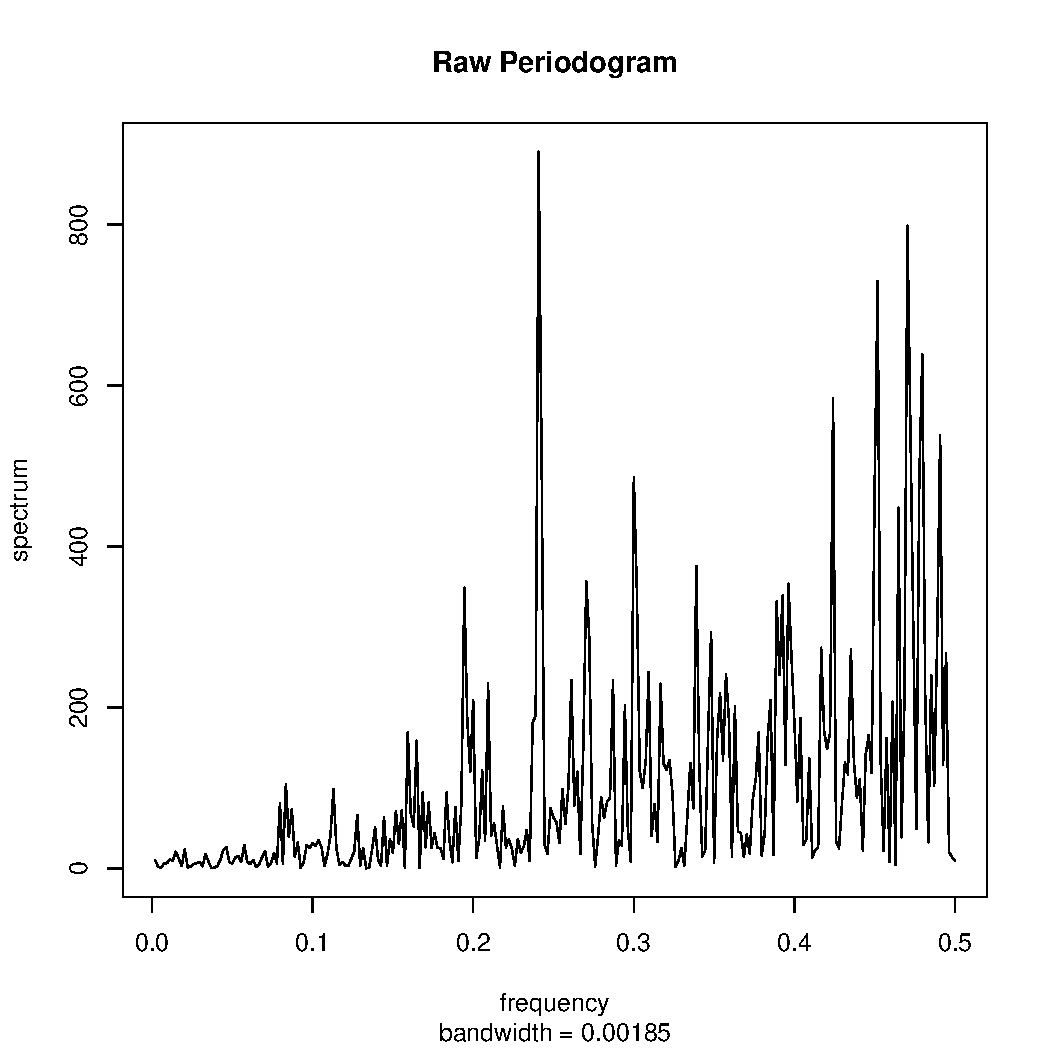
\includegraphics[width=0.45\linewidth]{../image/raw_periodogram.pdf}
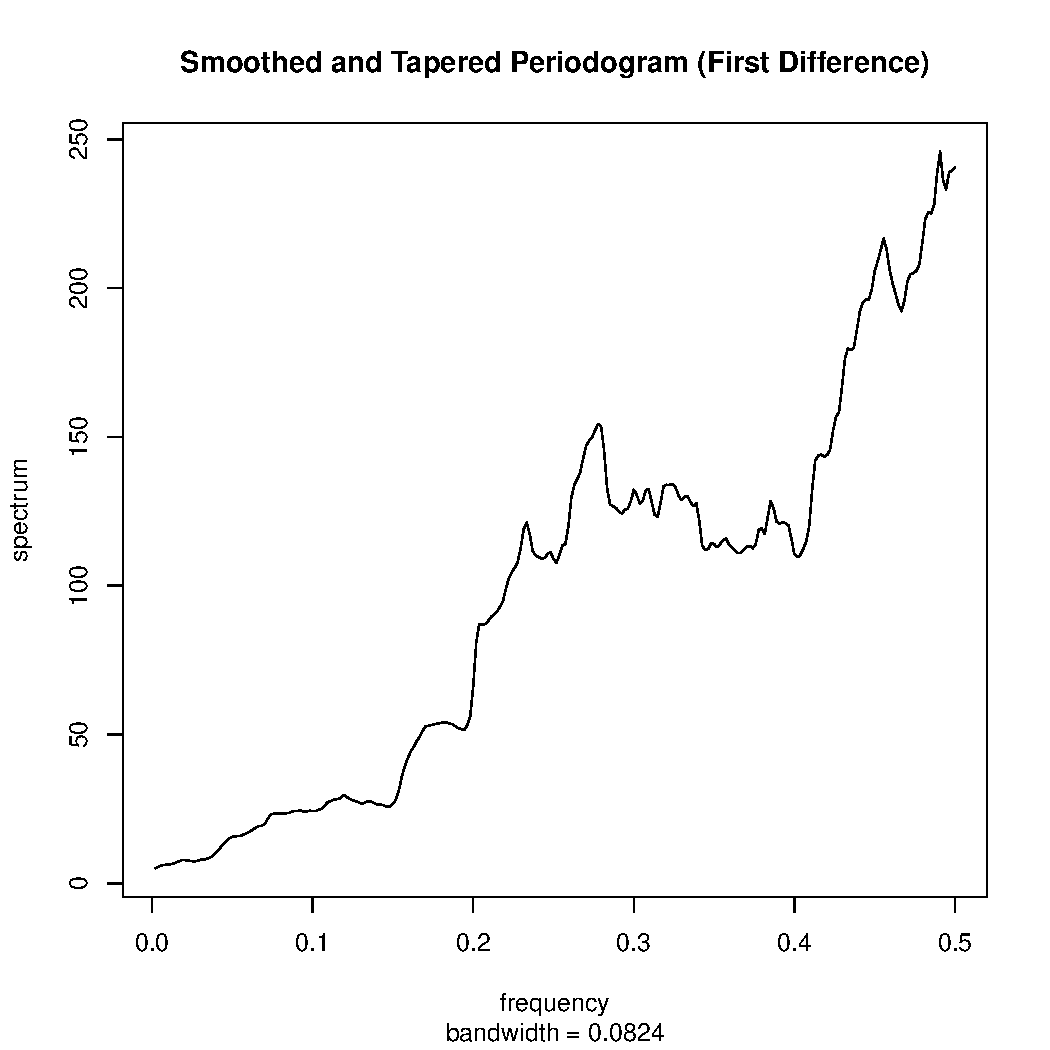
\includegraphics[width=0.45\linewidth]{../image/smooth_tapered_periodogram.pdf}
\caption{The Periodogram (left) and a Smoothed and Tapered periodogram (right) of the once differenced time series. Smoothed with a Modified Daniell Kernel with parameter $m = \sqrt{n} \approx 22$ and tapered with a split cosine bell taper with parameter $0.1$}
\label{periodogram}
\end{figure}



Upon visually inspecting our smoothed and tapered periodogram for our once differenced time series, we see a peak around $\omega = 0.27$, suggesting a seasonality in the data of $\frac{1}{0.27} \approx 4$. We later explore some models with this seasonal lag value. However, this bump is not apparent in the second differenced periodogram, which suggests that there may not be any important seasonality in the twice differenced dataset.

\subsection{Model Selection}
To evaluate how well our models fit the data, we compute the AIC, BIC, and AICc for each of our 12 candidate models, in table \ref{results}. We selected these 12 candidate models by playing around with the lower order options returned by the EACF for the once differenced and twiced differenced dataset. For each of the non-seasonal candidates we paired it with seasonal models with lag 4, where the seasonal $P$, $Q$, and $D$ were not too large. We also tried a seasonal lag of 3 on some models. We chose small values of $p$, $d$, $q$, $P$, $D$, and $Q$ because we noticed that many of the coefficients in higher order models were insignificant and had AIC, AICc, and BIC that were much larger than the corresponding smaller models. This leads us to conclude that larger order models may be overfitting to our training data set. We also tried to choose candidate models which had significant coefficients for a significance level of $\alpha = 0.05$ to be better ensure that we weren't overfitting to the training data. To aid model selection, we also calculate mean-squared error (MSE) for each of our candidate models. We calculate MSE in the following way:

\begin{algo}[MSE Calculation]
\begin{enumerate}
    \item for each year of data in validation:
    \begin{enumerate}
        \item prediction = forecast(1 year ahead, training_data)
        \item squared_error += $\| \text{prediction} - \text{year_of_data}\|_2^2$
        \item training_data = concatenate(training_data, year_of_data)
    \end{enumerate}
    \item MSE = squared_error / 3
\end{enumerate}
\end{algo}

Recall that our validation set consists of 3 years of data. So to calculate our MSE we predict one year ahead and take the sum of square difference between our prediction and what actually happened. We do this three total times for each of the 3 years in the validation and take the average. The averaging is useful to ensure that our model is generalizable to different forecasts and not to just a single one. We also could have performed a sum of square calculation 25 times instead of just 3 by performing a sum of square calculation on 12 month ahead forecasts starting from every month in the validation set that has 12 datapoints following it. We chose not to do this because we felt that the sum of square errors would be be too correlated with one another. A model that may only fit poorly for a portion of the overall validation set may get penalized repeatedly for it in this scheme. The AIC, AICc, BIC, and MSE for each of our candidate models is shown in table \ref{results}.

\begin{table}
\centering
\begin{tabular}{r || r | r| r| r}
$(p, d, q) \times(P, D, Q)_s$   & AIC   &AICc   &BIC    &MSE\\
\hline
$(0, 1, 1)$               & 5.248 &5.252  &4.265  &13212.18\\
$(0, 1, 1) \times (1, 0, 1)_4$   & 5.237 &5.241  &4.270  &13451.05\\ % Small p-values and passes ljung box p-values on seasonal ar1 and ma1; passes ljung box
$(0, 1, 1) \times (1, 1, 1)_4$   & 5.249 &5.254  &4.274  &13325.71\\
$(0, 1, 1) \times (1, 1, 2)_4$   & 5.242 &5.246  &4.275  &13728.1\\
\hline
$(1, 1, 2)$               & 5.256 & 5.260 &4.288  &13237.34\\
$(1, 1, 2) \times (1, 0, 1)_4$   & 5.243 &5.247  &4.292  &13785.23\\ %Large p-values on ma2, small 
$(1, 1, 2) \times (1, 1, 1)_4$   & 5.252 & 5.257 &4.294  &14144.5\\
$(1, 1, 2)\times (1, 1, 2)_4$   & 5.250 & 5.254 & 4.299 &13826.03\\
\hline
$(3, 2, 1)$             & 5.259& 5.263& 4.291 & 13216.42\\
$(3, 2, 1) \times (1, 0, 1)_4$ & 5.254& 5.258 & 4.303 &13664.76\\
\hline
$(0, 1, 1) \times (1, 0, 1)_3$ & 5.246 & 5.250 & 4.279 & 14670.6\\
$(3, 2, 1) \times (1, 0, 1)_3$ & 5.254 & 5.259 & 4.303 & 13456.07
\end{tabular}
\caption{The metrics associated with different SARIMA models denoted by the left hand column.}
\label{results}
\end{table}


Note that BIC tends to work better when the number of observations is large relative to the model order, and AICc does better when it is relatively smaller in comparison to the model order \cite{timeseriesanalysis}. In our project, the number of observations is quite large relative to the model order; for this reason, we decided to focus primarily on MSE and BIC values in determining our best model.

Hardly any of the models we considered in table \ref{results} failed the null hypothesis of Ljung-Box test with a significant $p$-value for any lag. In other words, the Ljung-Box test did not identify a statistically significant correlation among the sample residuals, for any of the models that we considered. This is promising, because we expect the sample residuals of a well-fitting model to be independent. Furthermore, the ACF of the residuals for nearly every model was statistically insignificant, which is indicative that the residuals of different observations are uncorrelated. However, the QQ-plot for nearly every model we considered indicated that our residuals do not look normally distributed. This might signify that a SARIMA model does not have the expressive power to capture some patterns that may be present in the dataset. This also causes any confidence interval (derived from a normal approximation) for forecast to potentially be unreliable. For the sake of brevity, we omit the Ljung-Box and QQ plots for the candidate models and only present them for the final model. The full results for all of our models can be found in our code on github\footnote{https://github.com/garyxcheng/terrorism_prediction/blob/master/sandbox.pdf}. A copy of the raw code is also in the appendix.

Based on our validation methods, we chose as an ARIMA(0, 1, 1) as our final model. Even though its AIC and AICc values are middle of the pack, it had the best BIC and MSE values. The full properties of this model is shown in Figure \ref{best_model} in the appendix. The MA coefficient on this model had a p-value of $\approx 0.0000$, and the model has non-significant residual ACF. Furthermore, it performs well on the Ljung-Box Statistic.




\subsection{Forecasting}

Using our final model, we generated a forecast of 12 months, displayed in Figure \ref{prediction}. The prediction fits the behavior of the data fairly well.  What actually occurred, shown in gray fits between the 2 standard error bars (which corresponds to $\approx 95\%$ confidence interval under a normal approximation) of the forecast.


\begin{figure}
\centering
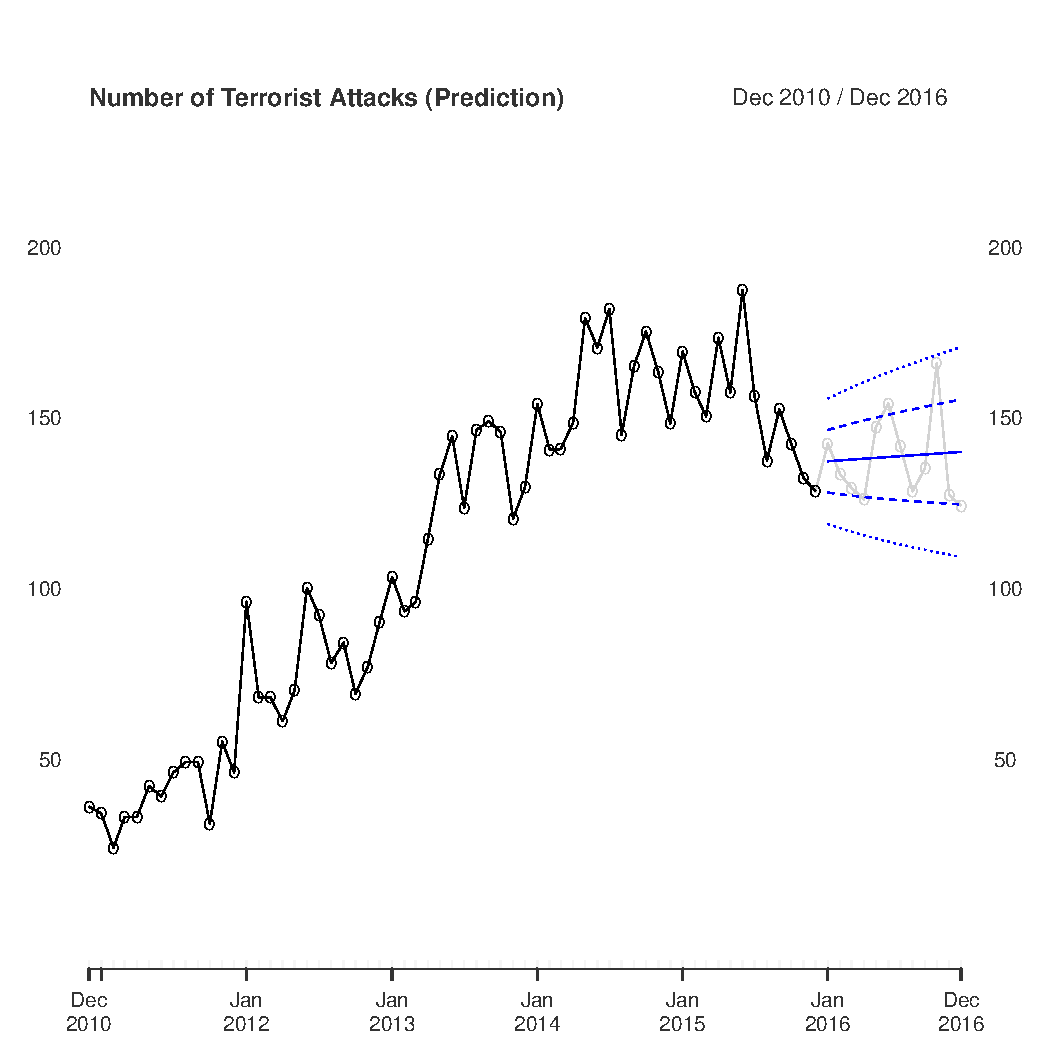
\includegraphics[width=0.75\linewidth]{../image/prediction_on_testing.pdf}
\caption{We use the model ARIMA(0, 1, 1) to generate a 12 month prediction denoted by the blue line. 1 standard error and 2 standard error bars are the blue dotted lines. What actually occured is shown by the light gray.}
\label{prediction}
\end{figure}


\section{Conclusion}
Through our analysis, we demonstrated that major terrorist attacks over a short period of time follow a predictable pattern. In particular, the ARIMA model we selected produced a reasonably accurate forecast of the monthly terrorist attacks in 2016.

Notably, our non-seasonal models fit the time series better than our seasonal models, which was an unexpected result. In fact, our final model was ARIMA(0, 1, 1), which is a fairly simple model. We suspect that considering data from all areas of the globe may have obscured seasonal and more complex, potentially non-linear patterns. In the future, filtering the data for a specific country or region may produce a more seasonal dataset. For example, incidents of terrorism in a given country may spike around election time, or during a specific season of the year.

Our next objective in analyzing the GTD would be to study its correlation to other datasets. Generally, terrorism attacks are motivated by an external cause, such as a collapse of a government or an ethnic conflict within a state. Therefore, studying the correlation between terrorist attacks over time and another time series would probably yield fruitful results. For example, we would expect that the GDP of a country and the number of terrorist attacks that occur in a country to be correlated.

This project was a good foray into the patterns in the GTD, but future research into filtered subsets of the GTD, as well as into exploring the relationship between the GTD and other datasets, is likely to produce novel results.

\printbibliography


\section{Appendix}
\begin{figure}[h]
\centering
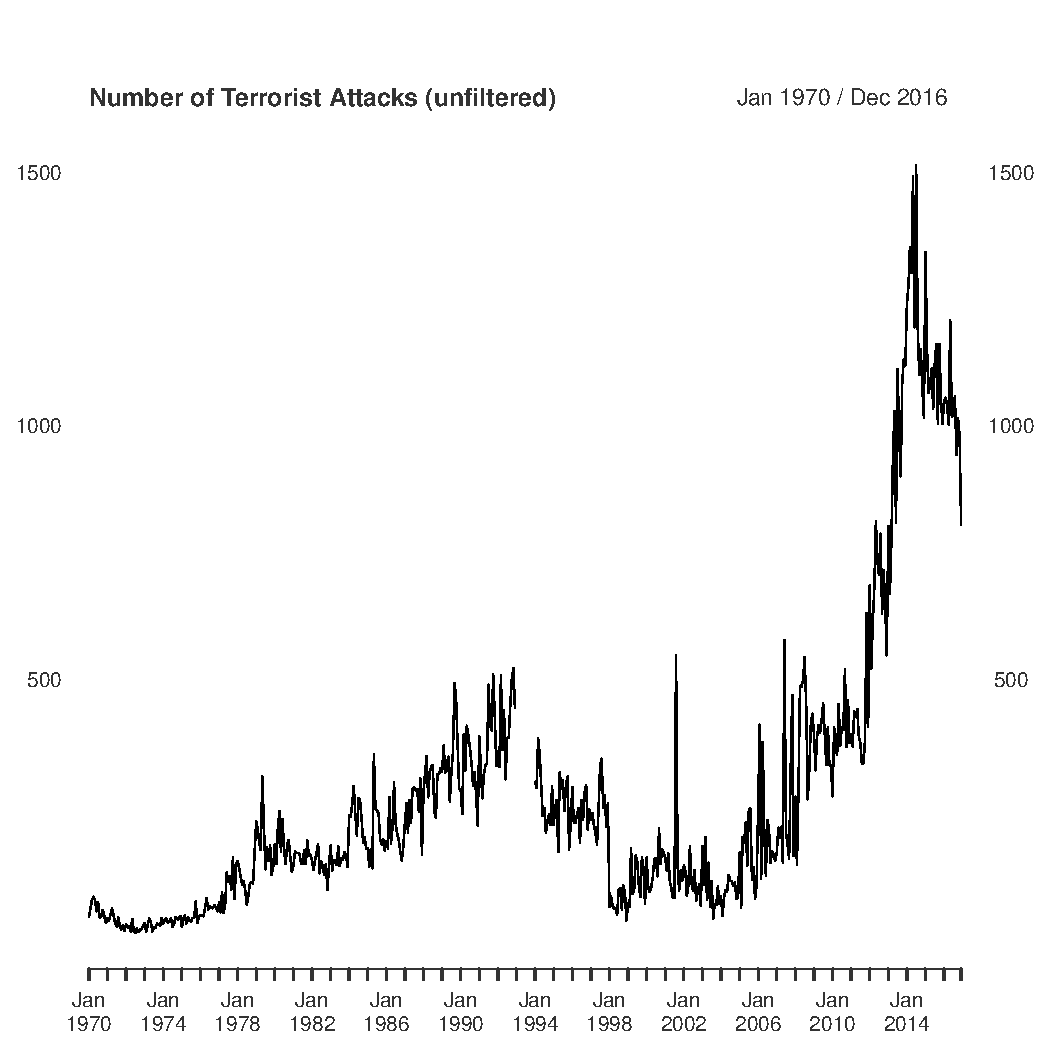
\includegraphics[width=0.75\linewidth]{../image/og_og_og.pdf}
\caption{The original time series of number of attacks per month from 1970 to 2016. Not filtered for Number of Casualities greater than or equal 10}
\label{ogogog}
\end{figure}

\begin{figure}[h]
\centering
    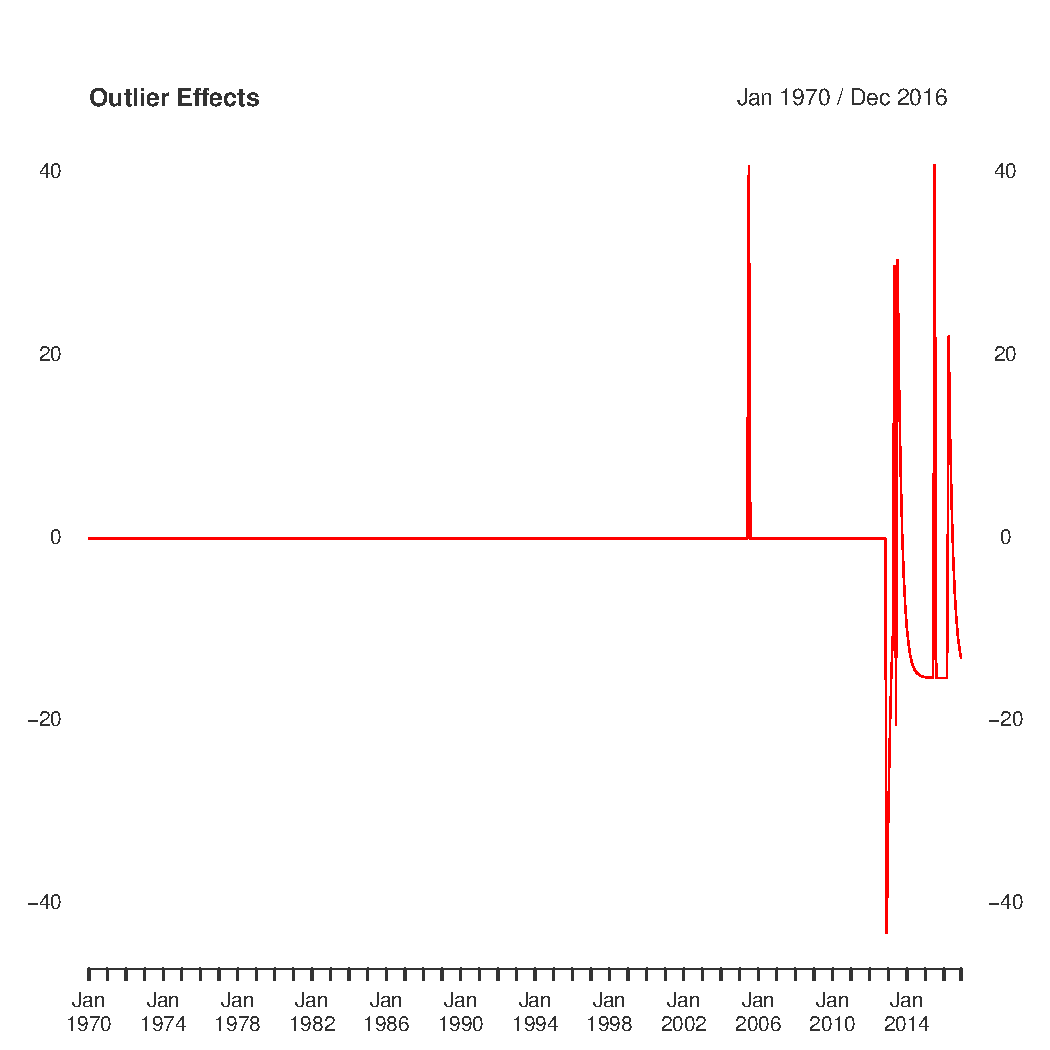
\includegraphics[width=0.75\textwidth]{../image/outlier_effects.pdf}
\caption{The outlier effects for each of the identitifed outliers are displayed here.}
\label{outlier_effect}
\end{figure}

\begin{figure}[h]
\centering
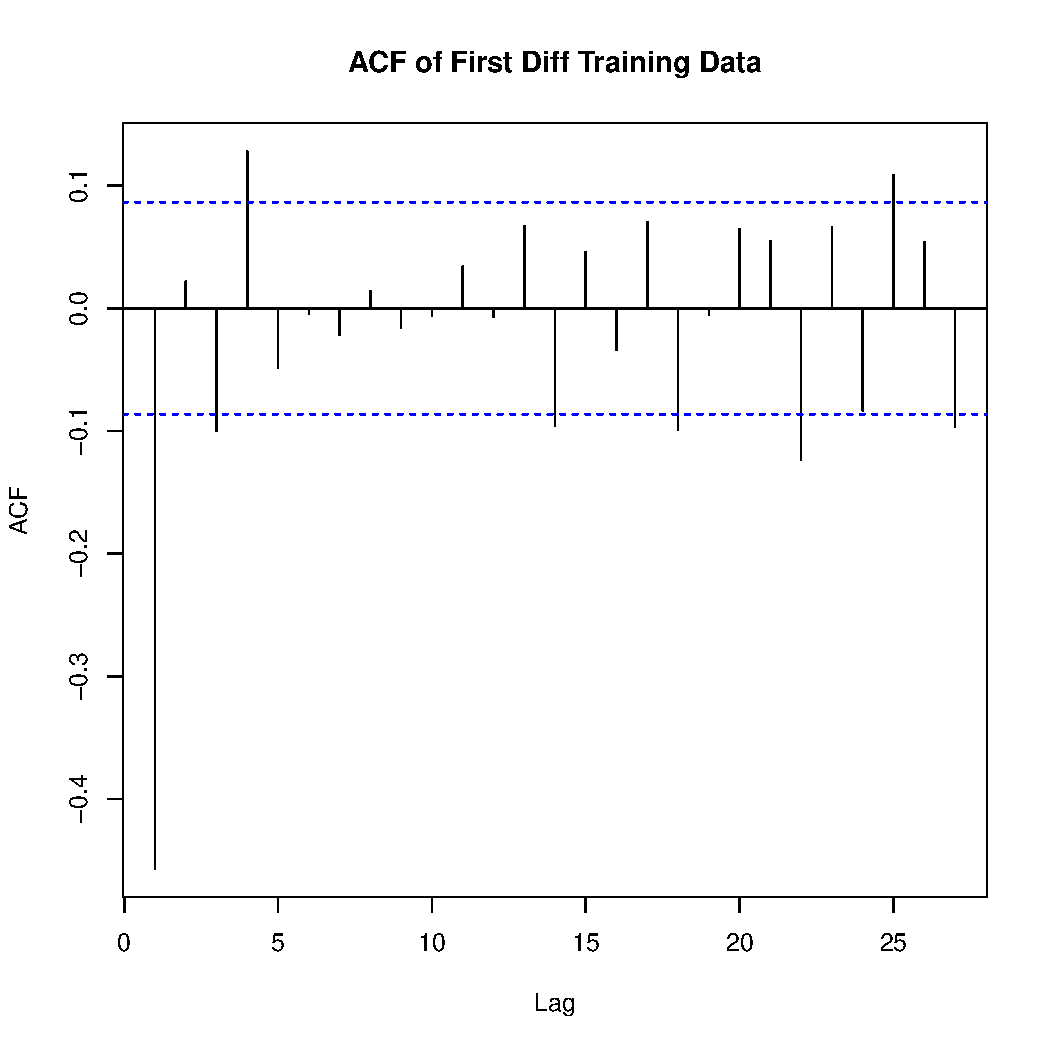
\includegraphics[width=0.45\linewidth]{../image/acf_first_diff.pdf}
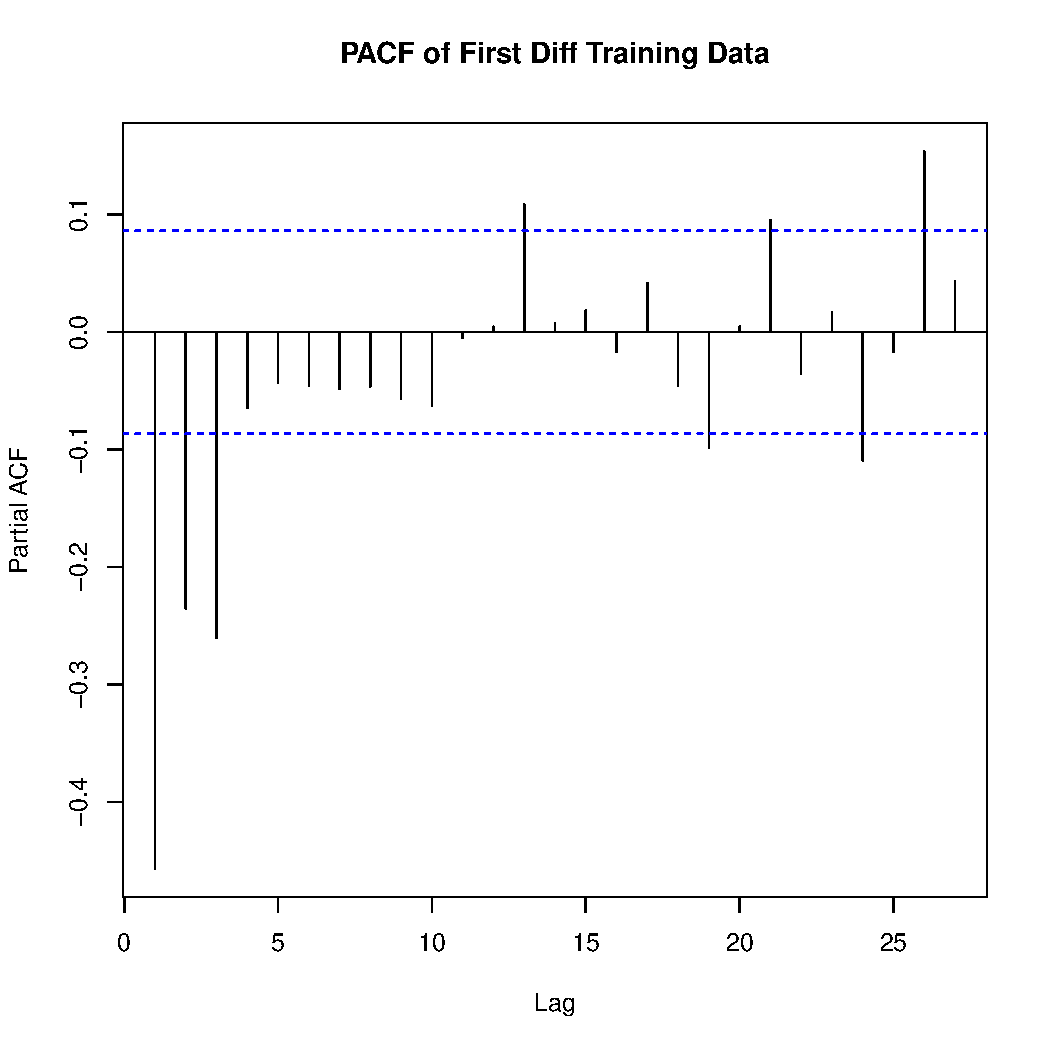
\includegraphics[width=0.45\linewidth]{../image/pacf_first_diff.pdf}
\caption{The ACF and PACF of the first diff time series}
\label{first_acf_pacf}
\end{figure}

\begin{figure}[h]
\centering
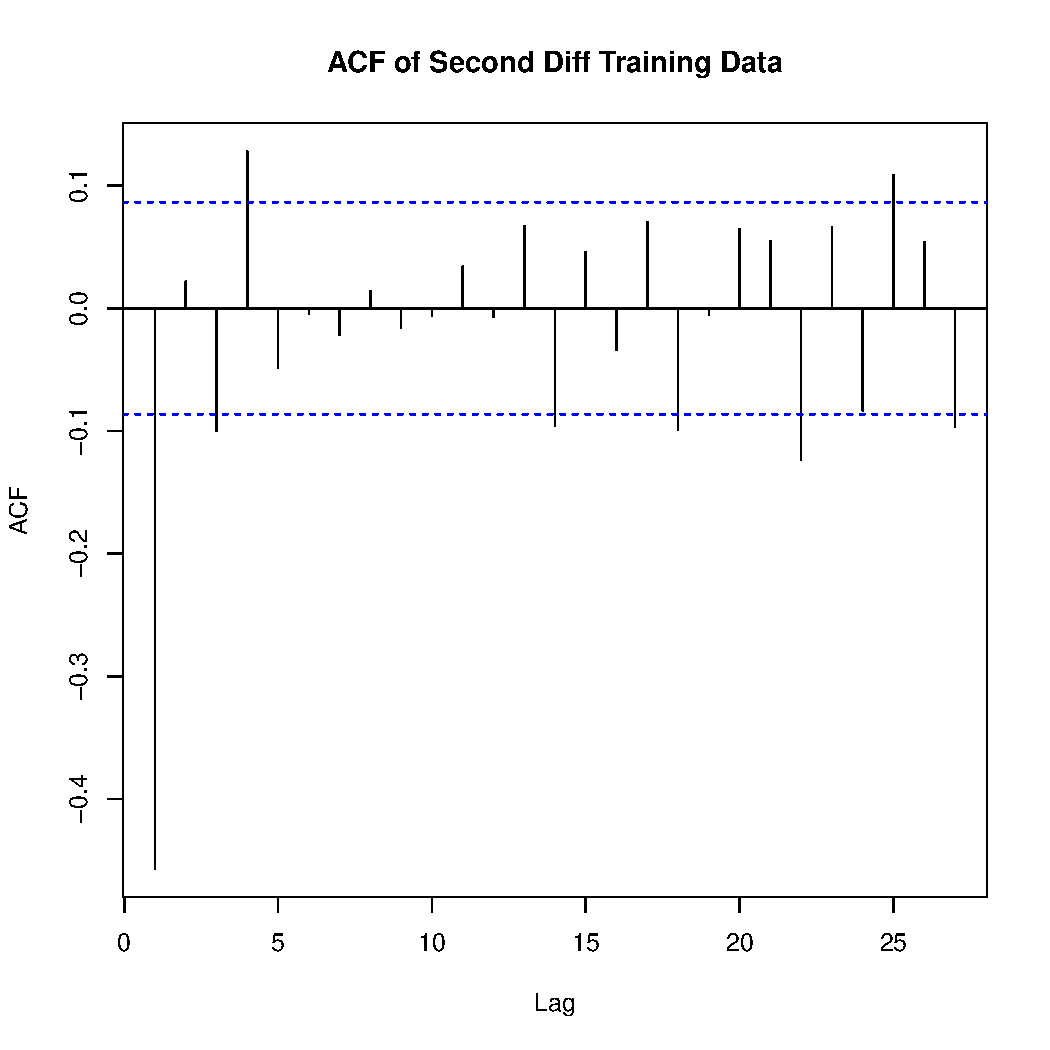
\includegraphics[width=0.45\linewidth]{../image/acf_second_diff.pdf}
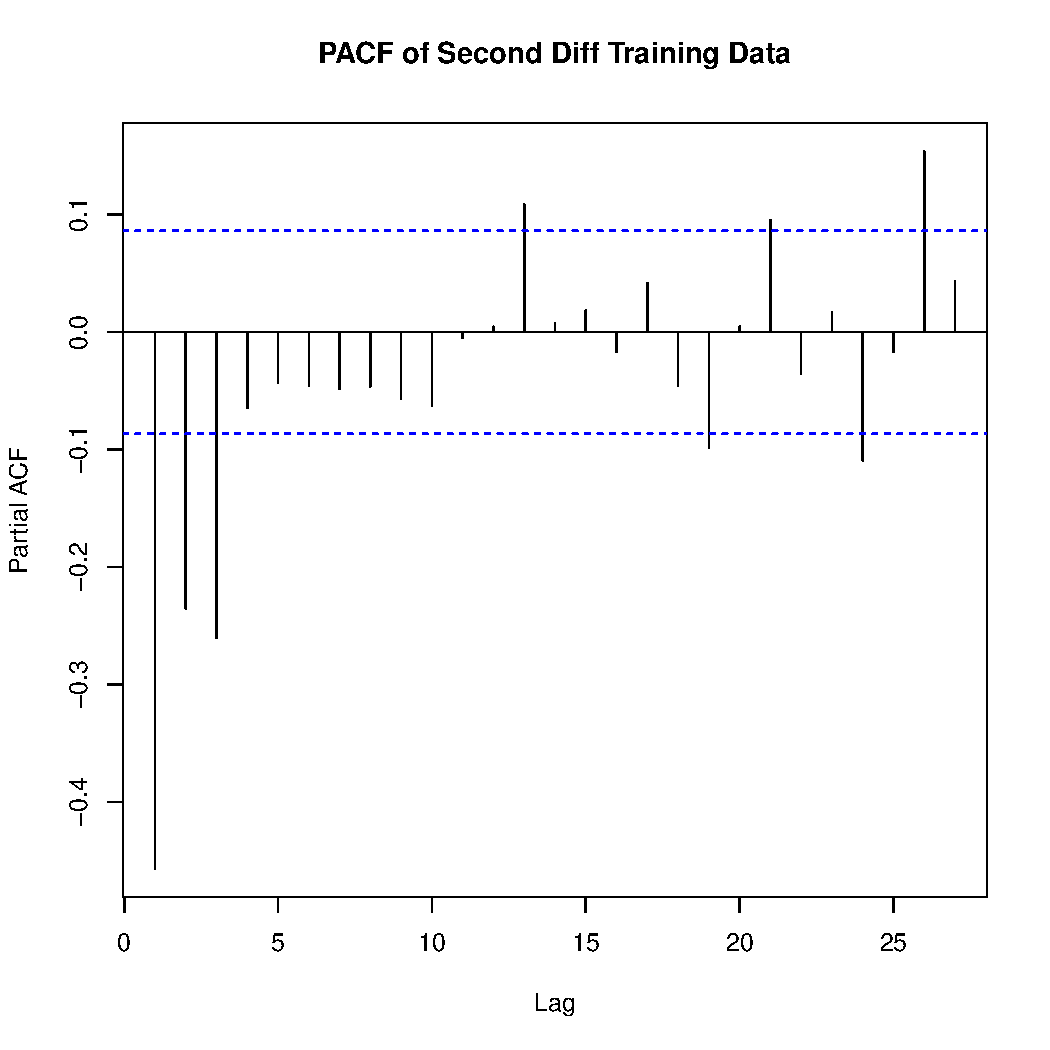
\includegraphics[width=0.45\linewidth]{../image/pacf_second_diff.pdf}
\caption{The ACF and PACF of the second diff time series}
\label{second_acf_pacf}
\end{figure}

\begin{figure}[h]
\centering
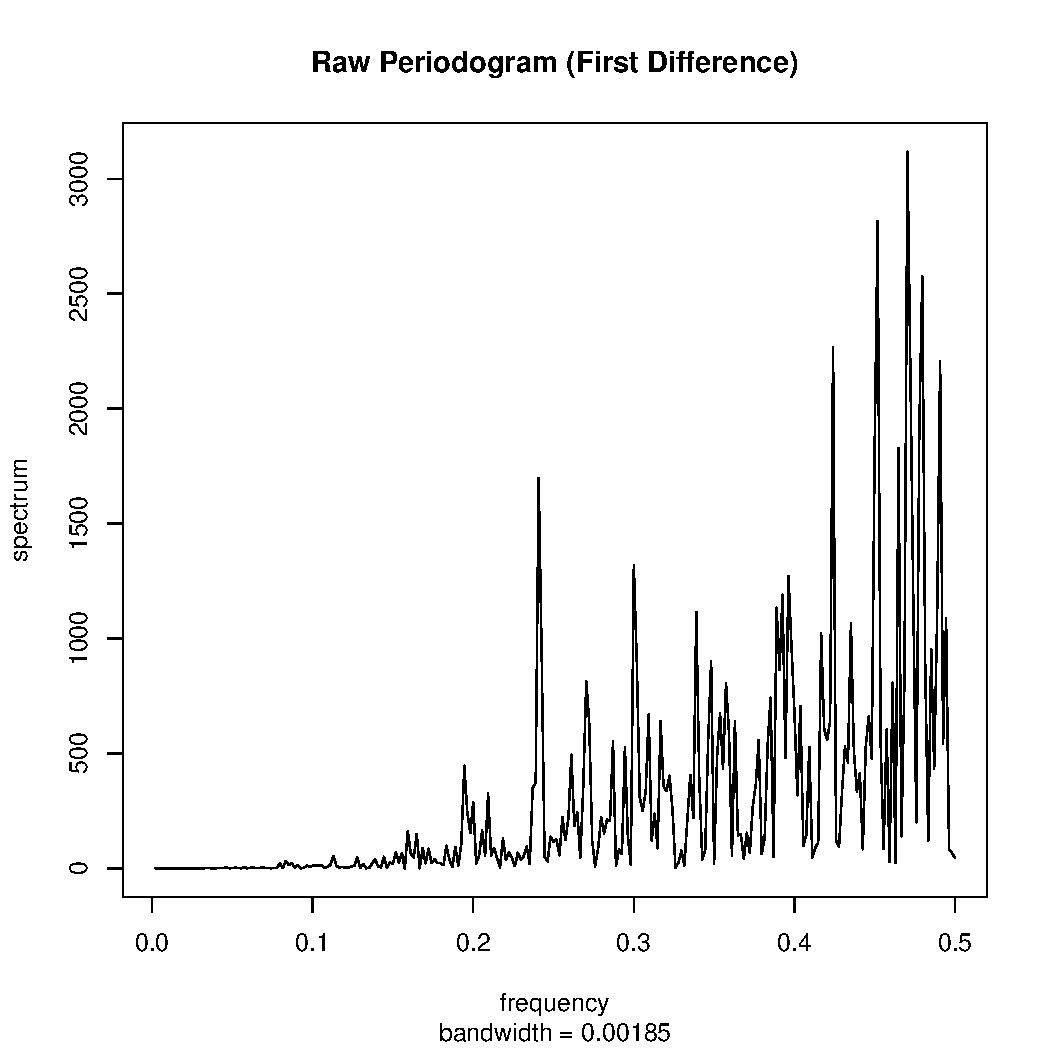
\includegraphics[width=0.45\linewidth]{../image/raw_periodogram_2.pdf}
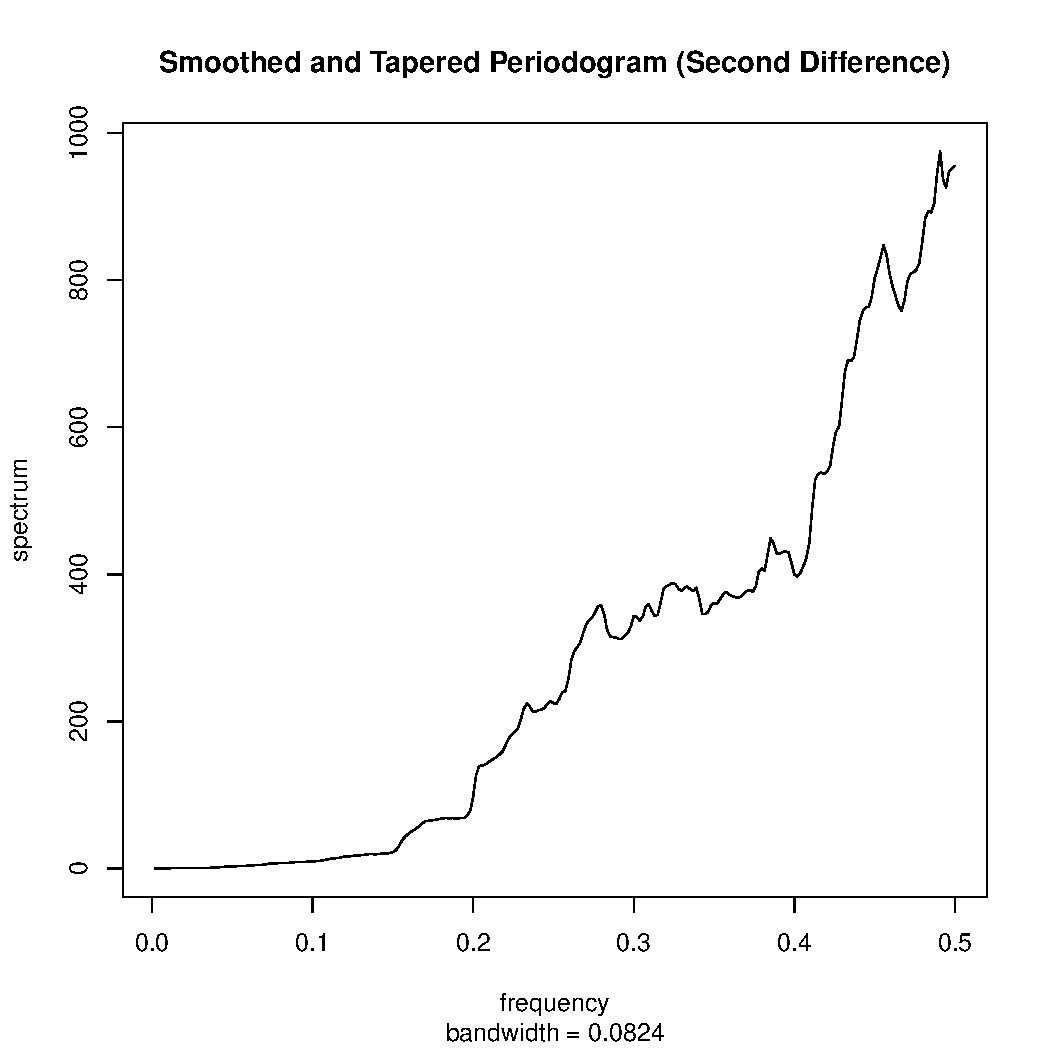
\includegraphics[width=0.45\linewidth]{../image/smooth_tapered_periodogram_2.pdf}
\caption{The Periodogram (left) and a Smoothed and Tapered periodogram (right) of the twice differenced time series. Smoothed with a Modified Daniell Kernel with parameter $m = \sqrt{n} \approx 22$ and tapered with a split cosine bell taper with parameter $0.1$}
\label{periodogram2}
\end{figure}

\begin{figure}[h]
\centering
    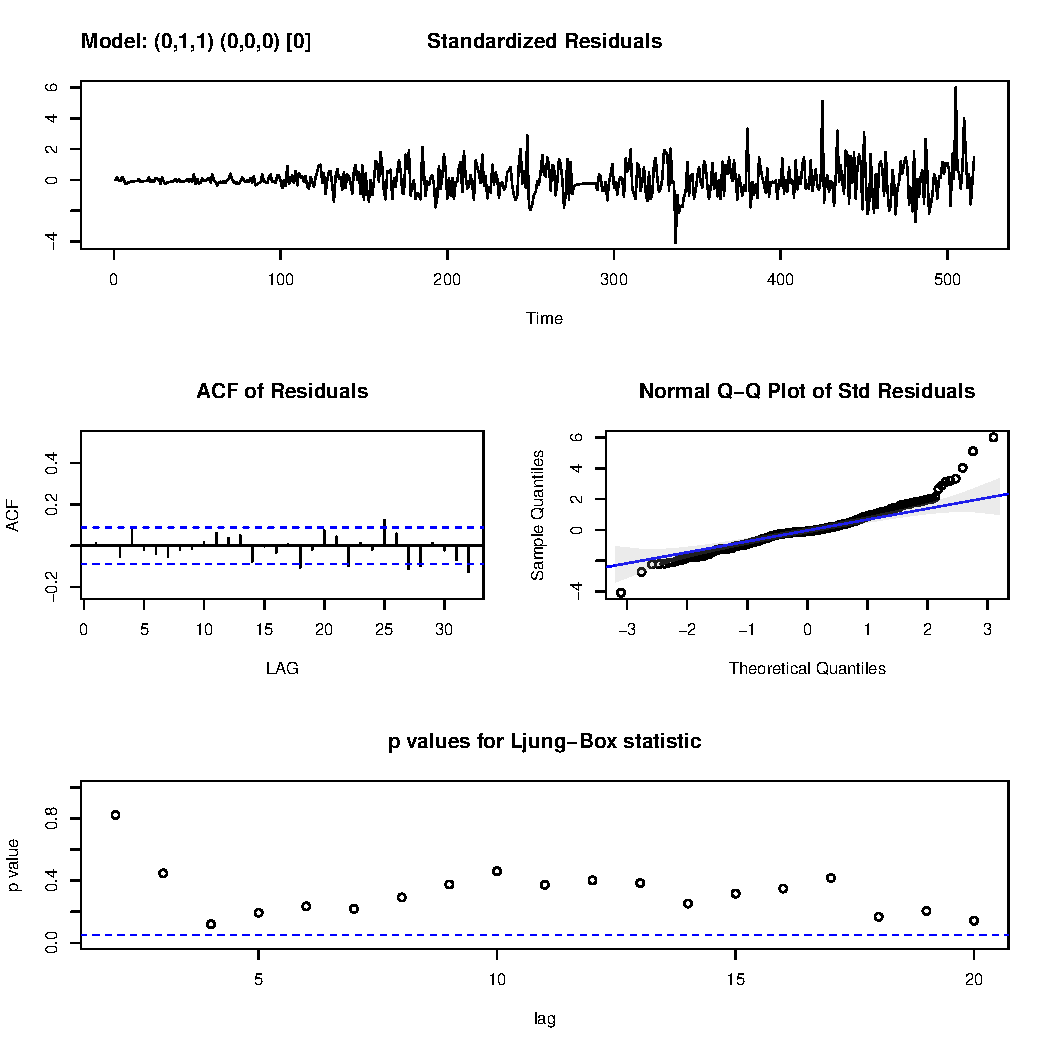
\includegraphics[width=0.75\textwidth]{../image/best_model.pdf}
\caption{This is the information from our best model.}
\label{best_model}
\end{figure}

\end{document} 